\chapter{Introduction}
\label{cha:introduction}

% mehr auf andere properties eingehen und weniger fairness -> fairness kann aber zum hinleiten zu dezentralität helfen

With the proliferation of new technologies, the amount of data will drastically increase and certainly empower new innovations. In fact, the worldwide interaction with data follows an exponentially growing trend, with a volume of 79 \acrfull{zb} in 2021, and an expected volume of 181 \acrshort{zb} in 2025 \cite{statistaDataWorldWide}. This giant pool of data can help companies to develop new business models, make better decisions through analytics and build smarter applications with machine learning models. For example, access to data can enhance the treatment of diseases in the healthcare sector \cite{koutsosAgoraPrivacyAwareData,wangBigDataAnalytics2018,suBDTFBlockchainBasedData2020} and increase productivity and efficiency in the agriculture sector \cite{elijahOverviewInternetThings2018}. More and more connected \acrfull{iot} devices accelerate the collection of valuable data \cite{ozyilmazIDMoBIoTData2018,lawrenzBlockchainTechnologyApproach2019}, however, without open and censorship-free access it cannot be used. Consequently, the economic value of data promotes the need for online data marketplaces \cite{dagevilleSnowflakeElasticData2016,krishnamachariI3IoTMarketplace2018}.

A conventional data marketplace is a two-party trading platform, where data owners, referred to as sellers \emph{S}, monetize valuable data to get compensated for data access by interested parties, referred to as buyers \emph{B} \cite{banerjeeBlockchainEnabledData2019}. Such conventional two-party data marketplaces have one thing in common -- it is not possible to guarantee fair exchange, i.e. receiving legitimate data as \emph{B} while receiving the agreed-upon payment as \emph{S}, without a Trusted Third Party (TTP) \cite{banerjeeBlockchainEnabledData2019}. Hence, the two-party model is typically extended by a centralized trading platform, where \emph{S} uploads and advertises his or her data, and the platform sells it on behalf of \emph{S} \cite{banerjeeBlockchainEnabledData2019,daiSDTESecureBlockchainBased2020,suBDTFBlockchainBasedData2020}.

% A conventional data marketplace is a two-party trading platform, where data owners, referred as sellers \emph{S}, monetize their valuable data to get compensated for data access by interested parties, referred as buyers \emph{B} \cite{banerjeeBlockchainEnabledData2019}. Such data marketplaces come in different variations. For example, there are paid subscription models for an interface to dynamic real-time data in contrast to a one-time-purchase model for access to a static resource. In addition, data marketplaces can be classified as Business-to-Business (B2B) or Business-to-Consumer (B2C) platforms. %Examples and citation or only citation?).
% However, all conventional two-party data marketplaces have one thing in common -- it is not possible to guarantee fair exchange, i.e. receiving legitimate data as \emph{B} while receiving the agreed-upon payment as \emph{S}, without a Trusted Third Party (TTP) \cite{banerjeeBlockchainEnabledData2019}. Hence, the two-party model is typically extended by a centralized trading platform, where \emph{S} uploads and advertises his or her data, and the platform sells the data on behalf of \emph{S} \cite{banerjeeBlockchainEnabledData2019,daiSDTESecureBlockchainBased2020,suBDTFBlockchainBasedData2020}.

Conventional data marketplaces are usually centralized platforms and hence, suffer from a variety of issues. A dishonest seller \emph{S} may be tempted to refuse access or return manipulated data after receiving the payment \cite{suBDTFBlockchainBasedData2020,lawrenzBlockchainTechnologyApproach2019}. On the opposite, a dishonest buyer \emph{B} may be tempted to never pay the price after receiving the purchased dataset \cite{lawrenzBlockchainTechnologyApproach2019}. Furthermore, a malicious platform might even take advantage of its own monopoly to advertise products and distort rankings for its own profit \cite{ramachandranDecentralizedDataMarketplace2018}. Even worse, a malicious platform has access to all advertised raw datasets \cite{banerjeeBlockchainEnabledData2019} and might resell them without \emph{S}'s knowledge \cite{serranoPeertoPeerOwnershipPreservingData2021,suBDTFBlockchainBasedData2020,daiSDTESecureBlockchainBased2020}.
%This is a form of piracy and, depending on the type of data, can violate privacy. All in all, a centralized platform is a \acrfull{spof} \cite{daiSDTESecureBlockchainBased2020} that is not able to satisfy \emph{Fairness}, \emph{Transparency}, \emph{Security}, \emph{Privacy}, and non-discrimination, among others \cite{banerjeeBlockchainEnabledData2019}. 
A decentralized infrastructure might help to reach all desirable properties \cite{ramachandranDecentralizedDataMarketplace2018}. Blockchain technology, first introduced in 2008 by Satoshi Nakamoto \cite{nakamotoBitcoinPeertoPeerElectronic}, provides a promising approach to that.

%Any digital data marketplace, whether centralized or decentralized, needs some specific key components and features. This includes: (i.) \emph{Fairness}; (ii.) \emph{Transparency}, \emph{Privacy} and \emph{Security}; (iii.) \emph{Regulation}; as well as (iv.) \emph{Efficiency}, according to Banerjee and Ruj \cite{banerjeeBlockchainEnabledData2019}. Ramachandran et al. \cite{ramachandranDecentralizedDataMarketplace2018} complements this by functional requirements such as: (v.) \emph{Posting and Discovery}; (vi.) \emph{Data Transfer and Payments}; (vii.) \emph{Metadata Organization}; (viii.) \emph{Data Quality - Buyer and Seller Ratings}; (ix.) \emph{Data Quality - Curation and Recommendations}; and (x.) \emph{Identity - and Access Control Management (IAM)}. These requirements are surrounded by the buyer and seller, as depicted in Figure \ref{fig:components}.

%\begin{figure}[!htb]
%    \centering
%    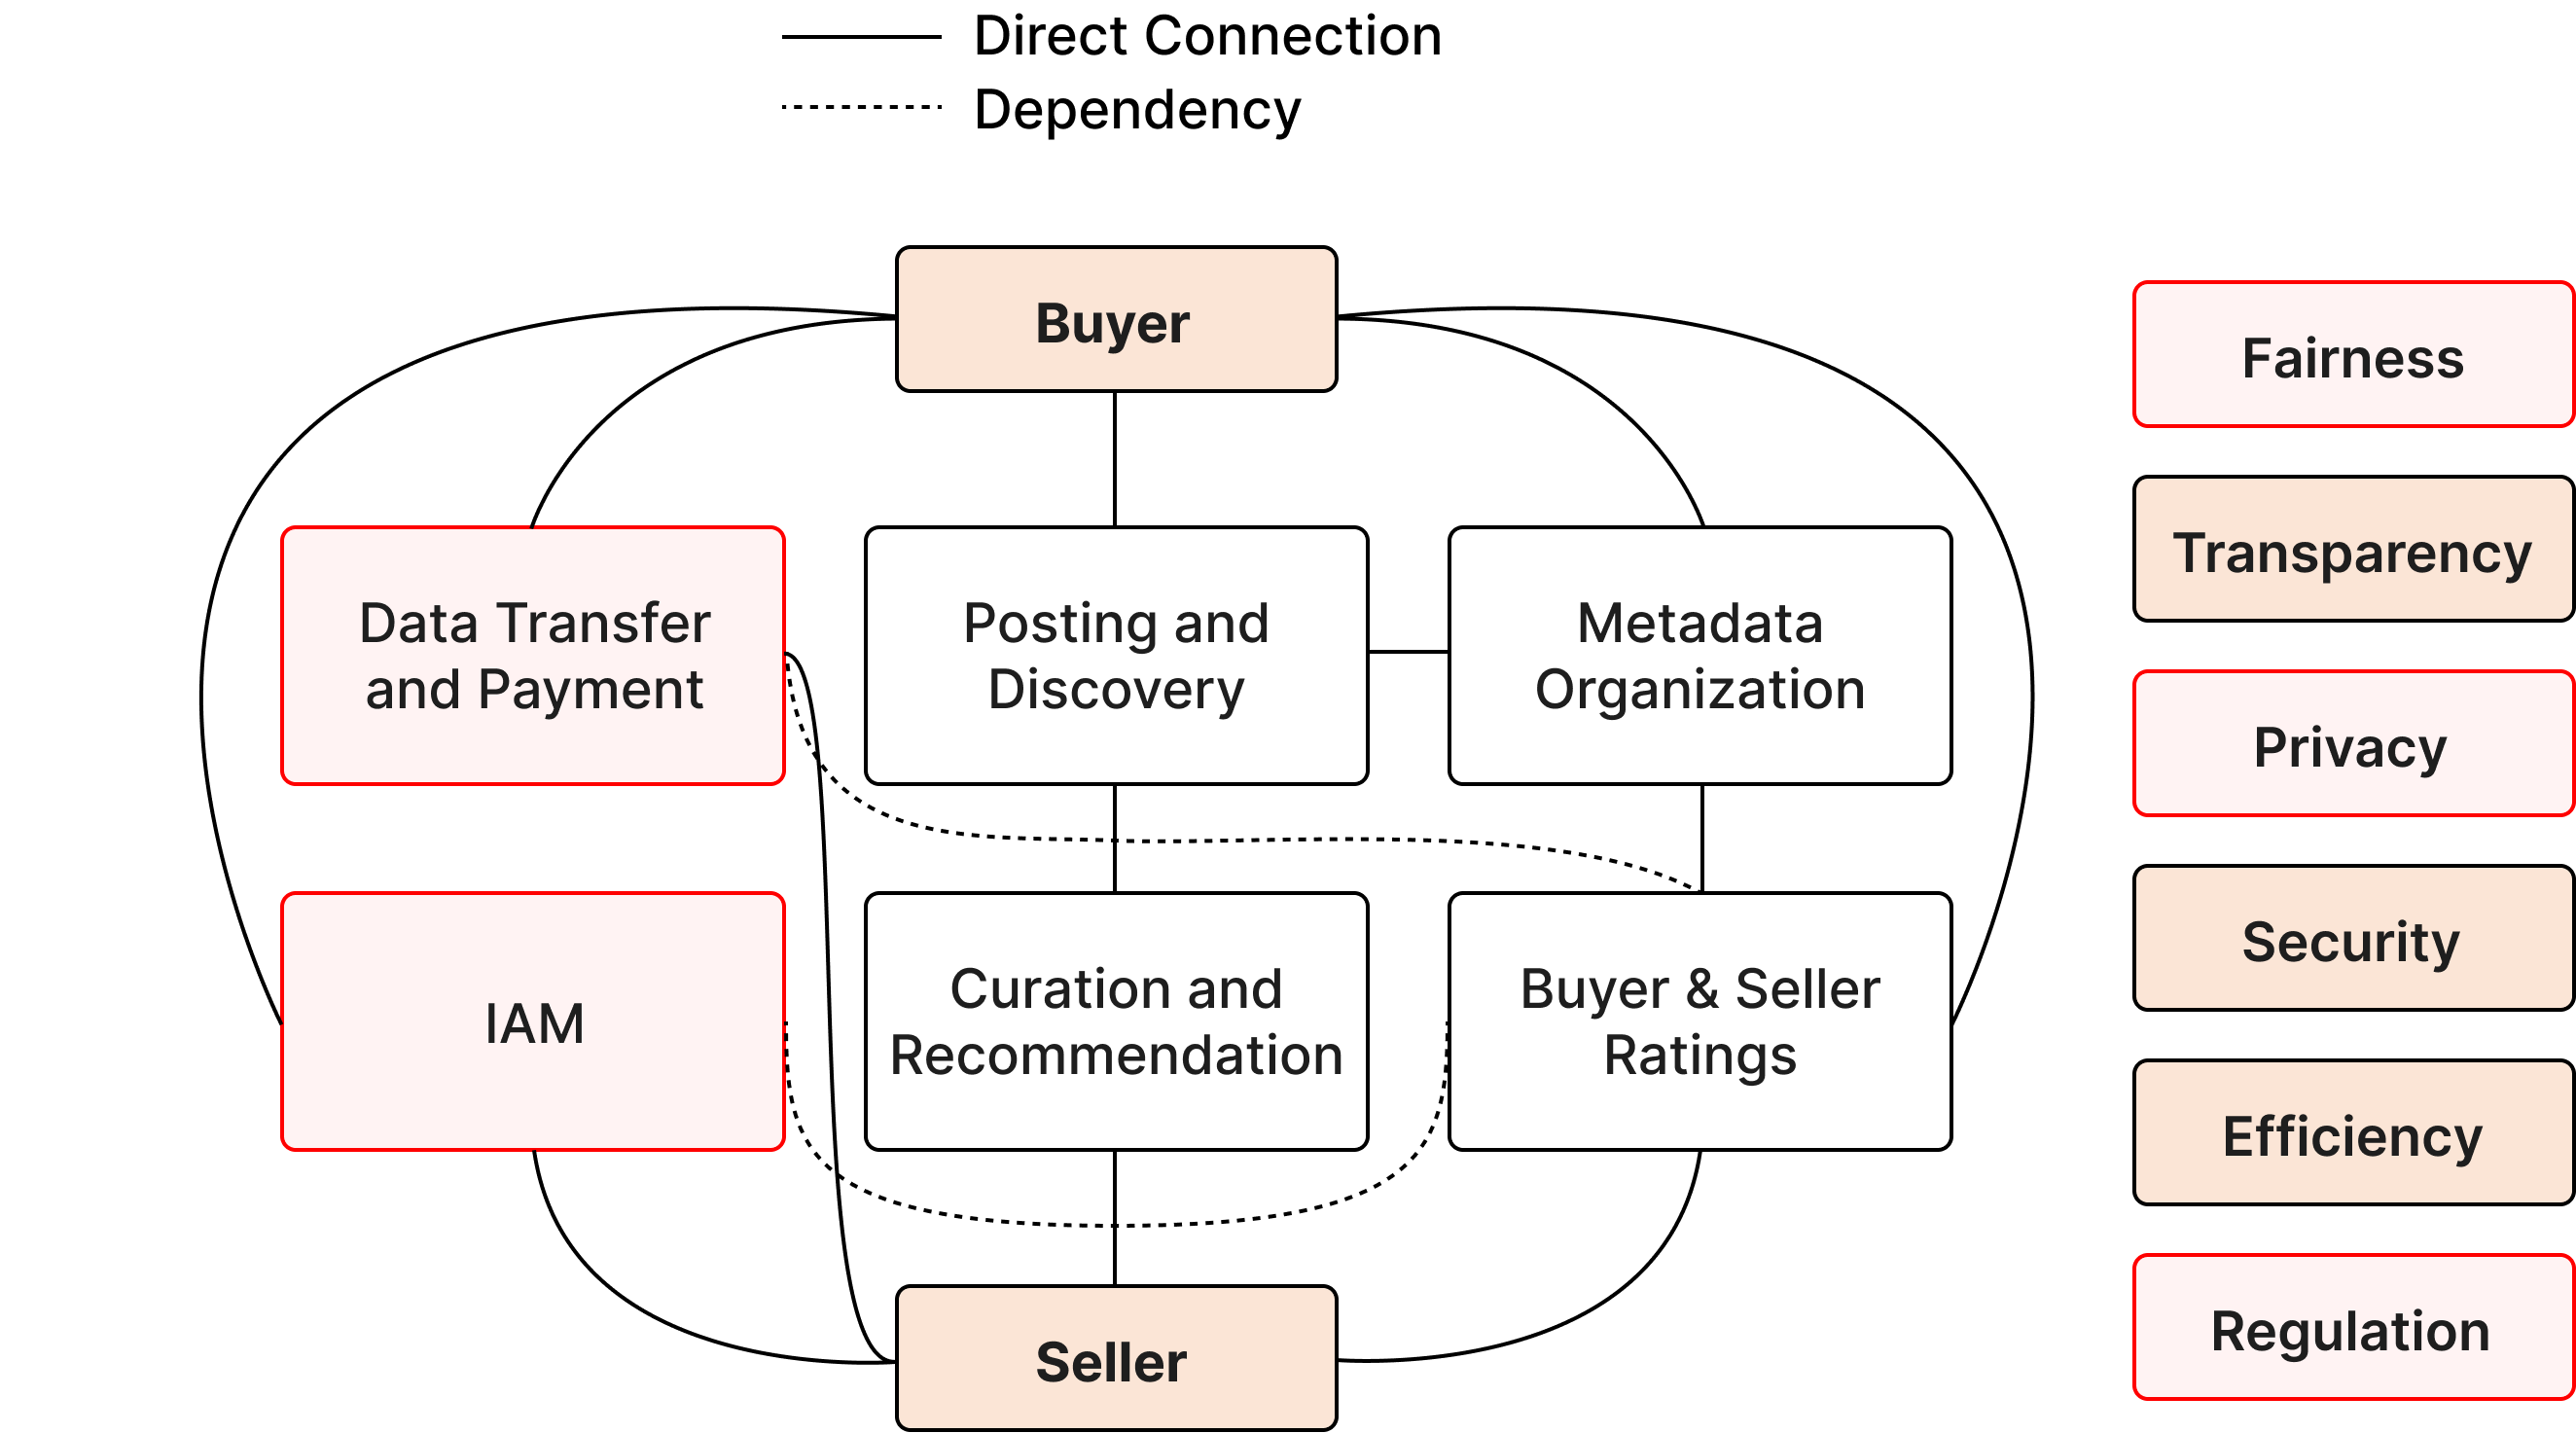
\includegraphics[width=13cm]{images/components.png}
%    \caption[Key components and features of a digital data trading platform]{Key components and features of a digital data trading platform. All components in red show the aspired enhancements by the contributions of this thesis.}
%    \label{fig:components}
%\end{figure}

"Blockchain-based application architectures benefit from a set of unique properties including immutability and transparency of cryptographically-secured and peer-recorded transactions, which have been agreed upon by network consensus" \cite{eberhardtBlockchainInsightsOffChaining2017}. According to that, it is trivial to implement sufficient \emph{Transparency} and \emph{Security} in blockchain-based data marketplaces. Furthermore, it turns out the non-trivial \emph{Fairness} problem in a two-party trading relationship seems to be solved by Blockchain technology in one atomic swap \cite{dziembowskiFairSwapHowFairly2018,liZKCPlusOptimizedFairexchange2021}. However, \emph{Privacy}, \emph{Regulation} and \emph{Efficiency} remains a bigger problem for blockchain-based data marketplaces due to limitations of public permission-less Blockchains such as Bitcoin \cite{nakamotoBitcoinPeertoPeerElectronic} and Ethereum \cite{buterinNEXTGENERATIONSMART}.

%Public permission-less Blockchains inherently validate and process transaction data at every node, in order to guarantee network consensus. By virtue of its design, all data is available at each node which makes this system purposely public in favor of transparency properties. However, data sharing often incorporates \acrfull{pii} and confidential data. Consequently, storing and computing private data on these ledgers is conflicting with Privacy requirements, enforced by regulations such as the \acrfull{gdpr} \cite{european_commission_regulation_2016}. In any case, it is not advisable to store large amounts of data in Blockchains due to block-size limitations, Blockchain bloating and extremely high associated storage costs.

%Off-chain storage solutions are suggested to overcome this limitation. In particular the Content-Addressable Storage Pattern \cite{eberhardtBlockchainInsightsOffChaining2017} seems to be a reasonable solution to store large amounts of data while keeping key properties of Blockchains such as immutability. Decentralized peer-to-peer networks such as IPFS \cite{benetIPFSContentAddressed2014}, Filecoin \cite{filecoin} and SWARM \cite{swarm} provide a promising approach to that. However, these networks suffer from the same Privacy issues as Blockchains due to open access and data replication across the network.

Another problem seems to be the enforcement of access and usage regulations in a distrusted setting without a \acrfull{ttp}. A seller loses full control over his data when the buyer receives it. Hence, he or she is not able to enforce geographical usage restrictions or purpose limitations for example. This especially violates the principle of purpose limitation codified in Art. 5 of the \acrshort{gdpr} \cite[Art. 5 (1 b)]{european_commission_regulation_2016}. Given a malicious buyer, he or she might even resell the purchased dataset without the seller's knowledge.

\noindent We observe, that most of the problems occur when data leaves the boundaries of the seller, i.e. a raw dataset is moved to a storage platform and/or moved to the buyer, to be processed subsequently. While data encryption might solve the problem in the first place, \emph{Regulation} and \emph{Privacy} still remain a problem, when the buyer decrypts the raw dataset. Accordingly, we suggest flipping the strategy, i.e. raw datasets never leave the boundary of the seller and only an aggregated computation over the dataset is moved to the buyer, thereby protecting \acrshort{pii} and confidential data. This paradigm is referred to as \emph{Compute-to-Data}. However, a problem with this paradigm is that, given a malicious seller, the buyer cannot verify if the result has been computed correctly. This leads to the following research questions:
%Verifiable Off-chain Computation (VOC) has been suggested to address this problem \cite{eberhardtOffchainingModelsApproaches2018,eberhardtBlockchainInsightsOffChaining2017}.

%This thesis focuses on \emph{Privacy}, \emph{Fairness} and \emph{Regulation} enhancements in blockchain-based data trading platforms, by combining Compute-to-Data with Verifiable Off-chain Computation (VOC). It implicitly targets the \emph{Data Transfer} and \emph{Payment} process as well as \emph{IAM} -- some of the fundamental functional requirements, as depicted in Figure \ref{fig:components}.

Thereby, we make two individual contributions ...:

This thesis presents the implementation of a practical real world data marketplace for verifiable statistical computations on private datasets. It addresses \emph{Privacy}, \emph{Fairness} and \emph{Regulation} problems of blockchain-based data trading platforms, while the focus is on \emph{Privacy}. \emph{Furthermore, I only focus on static tabular datasets with very infrequent changes. Hence, I do \textbf{not} focus on real-time streaming data and training of machine-learning models}. My proposed implementation implicitly targets the \emph{Data Transfer} and \emph{Payment} process as well as \emph{IAM} -- some of the fundamental functional requirements, as already depicted in Figure \ref{fig:components}. Specifically, I construct a secure blockchain-based data trading ecosystem, using Blockchain as a medium to (i.) prevent single-point of failure; (ii.) define data usage policies; (iii.) create a transparent, non-repudiable and tamper-proof log of transactions; and (iv.) enforce a fair data exchange protocol. However, the \emph{focus} of this thesis is rather on creating a generic mechanism to make a variety of computations on arbitrary private datasets verifiable, and Blockchain is a necessary part of the puzzle. This thesis uses Verifiable Off-chain Computation (VOC) to address this problem \cite{eberhardtOffchainingModelsApproaches2018,eberhardtBlockchainInsightsOffChaining2017}.

%weitere problems je nach art des marketplaces
\begin{enumerate}
    \item What components are mandatory for a blockchain-based data trading platform and how can the Compute-to-Data paradigm be applied?
    \item How can the Compute-to-Data paradigm be made verifiable without sacrificing privacy?
    \item How practical is the proposed solution?
\end{enumerate}

The remainder of this thesis is organized as follows: Chapter \ref{cha:background} provides fundamental background knowledge to understand the remainder of this thesis. Chapter \ref{cha:relatedwork} gives a brief overview of the current research, with regard to privacy-aware blockchain-based data marketplaces. Chapter \ref{cha:requirements} summarizes the functional and non-functional requirements for the desired outcoming software artifact. The concept \& design of the software artifact is outlined in Chapter \ref{cha:cod} and its implementation explained in Chapter \ref{cha:implementation}. Lastly, Chapter \ref{cha:evaluation} evaluates and discusses the implementation based on the defined requirements, followed by a conclusion in Chapter \ref{cha:conclusion}, to summarize the results and ideas for future work.